\chapter{Sistemas de Arquivos}
Em um computador, os dados podem ser armazenados em vários dispositivos físicos diferentes como disco flexível, fita, disco rígido, CD, etc.. Para simplificar o tratamento, o SO fornece uma visão lógica e uniforme do sistema de armazenamento e uma visão lógica do armazenamento em si, sendo ela o arquivo.

O sistema de arquivo será o módulo do SO responsável pela criação da abstração de arquivos e por seu gerenciamento.

\section{Arquivos}
\begin{definicao}{Arquivo}
  Coleção de dados relacionados entre si
\end{definicao}

Cada arquivo possui um nome, que o identifica. Além do nome, o arquivo possui outros atributos como tipo, nome do criador, tamanho, etc.. As informações contidas em um arquivo geralmente são \textbf{persistentes} e armazenadas em dispositivos não-voláteis.

\subsection{Estruturação}
O servidor de arquivos deve implementar a abstração de arquivo para o restante do sistema. Para tal, ele deve determinar como o arquivo será estruturado internamente. As estruturas mais comuns são: sequências de \textit{bytes}, sequência de registros e árvore de registros, ilustradas na Figure \ref{fig:file-structures}.

\begin{figure}[h]
  \centering
  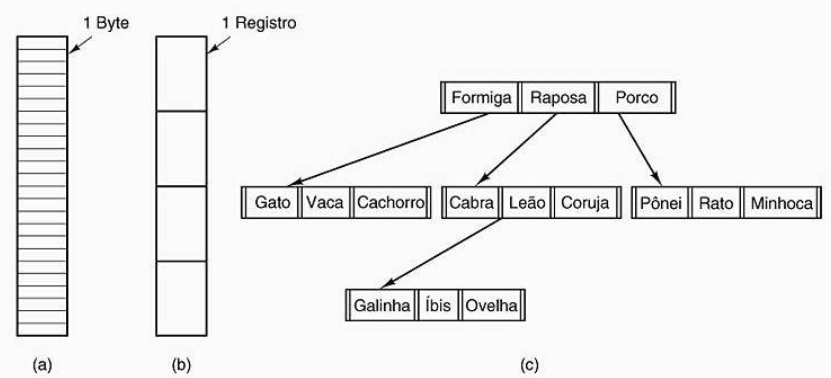
\includegraphics[width=.8\textwidth]{file-structures}
  \caption{As diferentes estruturas de arquivo: (a) sequência de \textit{bytes} (b) sequência de registros e (c) árvore de registros}
  \label{fig:file-structures}
\end{figure}

\subsection{Tipos}
Cada sistema de arquivos determina os tipos de arquivos suportados por ele. Sistemas como o Unix ou o DOS suportam os seguintes tipos:

\begin{itemize}
  \item \textbf{Arquivos Regulares:} contém os dados do usuário;
  \item \textbf{Arquivos Diretório:} arquivos utilizados na manutenção do sistema de arquivos;
  \item \textbf{Arquivos Especiais:} arquivos ligados a dispositivos de E/S.
\end{itemize}


\subsection{Atributos}
Além do nome e dos dados, o SO associa a cada arquivo um conjunto de infomações que auxiliam na ferência dos mesmos. Estas informações adicionais são chamadas atributos e estão geralmente contidas na tabela de arquivos. São exemplos de atributos:

\begin{itemize}
  \item \textbf{Proteção}: indica as permissões de acesso ao arquivo;
  \item \textbf{\textit{Password}:} senha necessária para o acesso ao arquivo;
  \item \textbf{Criador:} usuário criador do arquivo;
  \item \textbf{\textit{Owner}:} proprietário atual do arquivo;
  \item \textbf{\textit{Flag} de oculto:} impede que o nome do arquivo apareça na lista de arquivos;
  \item \textbf{\textit{Flag} de temporário:} o arquivo é deletado quando o processo que o criou morrer;
  \item \textbf{Tamanho:} tamanho atual do arquivo;
  \item \textbf{Tamanho máximo:} tamanho máximo que o arquivo pode atingir;
  \item Instante da última modificação e da criação;
\end{itemize}





\section{Operações sobre Arquivos}
As operações sobre arquivos geralmente levam em consideração um conjunto de entidades de um sistema de arquivos, sendo elas:

\begin{itemize}
  \item \textbf{Tabela de Arquivos:} uma tabela global do sistema, onde existe uma entrada para cada arquivo, contendo as informações referentes a cada um;

  \item \textbf{Diretório:} caminho que leva ao arquivo. Ao ser criado, o arquivo é posicionado em um diretório e a tabela de arquivos deste diretório deve conter uma entrada para o novo arquivo;

  \item \textbf{Tabela de Arquivos Abertos por Processo}: tabela criada para cada processo, sendo indexada pelo descritor de arquivos. Cada entrada referencia um arquivo aberto pelo processo, indicando a sua posição corrente no arquivo, permissões de acesso, etc.. Quando o processo morre, essa tabela deixa de existir;

  \item \textbf{Descritor de Arquivo:} índice que referencia uma entrada na tabela de arquivos abertos do processo. Operações a serem realizadas no arquivo devem ser feitas utilizando este descritor, requisitado ao SO pelo processo;

  \item \textbf{Posição Corrente:} ponteiro que indica qual a posição do arquivo será acessada na próxima vez. As operações de leitura e escrita incrementam o valor da posição corrente do arquivo do número de \textit{bytes} lidos e escritos.
\end{itemize}

% TODO: ILUSTRAR COM IMAGENS DO TANENBAUM
Agora definimos as operações sobre os arquivos:

\subsubsection{\textit{Create}}
Operação de criação de um arquivo. Deve-se criar uma entrada para o novo arquivo no diretório especificado. Além disso, cria-se uma entrada na tabela de arquivos com o nome do criador, data de criação e permissões de acesso. O arquivo recém-criado não possui dado algum.


\subsubsection{\textit{Delete}}
Libera o espaço ocupado pelo arquivo e deleta a entrada do diretório que aponta para o arquivo e a entrada do arquivo na tabela de arquivos.


\subsubsection{\textit{Open}}
Antes de ser utilizado, o arquivo precisa ser aberto. Esta chamada cria o \textit{link} entre a entrada do processo solicitante na \textit{tabela de processos} e a entrada do arquivo solicitado na \textit{tabela de arquivos}. Dessa forma, ele retorna um \textit{descritor de arquivos}, que será utilizado em todas as operações subsequentes sobre o arquivo. Ele também serve de índice na entrada da \textit{tabela de arquivos abertos do processo} requisitante, contendo informações sobre o descritor.

\begin{figure}[h]
  \centering
  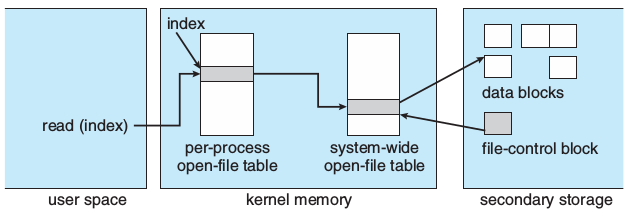
\includegraphics[width=.85\textwidth]{file-open-read}
  \caption{Figura que mostra como a operação \textit{read} utiliza as estruturas criadas na operação \textit{open} no contexto de arquivos}
  \label{fig:file-open-read}
\end{figure}

\subsubsection{\textit{Close}}
Esta operação desfaz o \textit{link} explicado anteriormente, removendo a entrada do descritor do arquivo solicitado da \textit{tabela de arquivos abertos do processo}. Todos os acessos subsequentes ao descritor e arquivo serão invalidados.


\subsubsection{\textit{Read}}
Para ler um arquivo, o processo deve especificar um descritor válido, a quantidade de dados a serem lidos e um local em memória (\textit{buffer}) onde os dados lidos devem ser colocados. A maioria das operações de leitura começam a partir de uma posição corrente.

\subsubsection{\textit{Write}}
Para escrever dados em um arquivos, o processo deve especificar um descritor válido, um \textit{buffer} local que contenha os dados a serem escritos e o tamanho destes dados. Normalmente, os dados são escritos em um arquivo a partir da posição corrente.

\subsection{Manipulação de Arquivos}
Podemos citar:
\begin{itemize}
  \item Criar arquivo;
  \item Abrir o arquivo;
  \item Ler, escrever, operações de \textit{append} e \textit{seek};
  \item Fechar o arquivo;
  \item Deletar o arquivo.
\end{itemize}










\section{Diretórios}
Diretórios são utilizados para auxiliar a disposição dos arquivos no sistema de arquivos. São estruturas hierárquicas, com uma entrada por arquivo. Cada entrada guarda o nome do arquivo, seus atributos e os endereços do disco onde ele está.







\section{Implementação de Arquivos}
A primeira decisão na implementação de arquivos é como os mesmos serão armazenados em blocos de disco. Para a associação de blocos de disco a arquivos, temos três abordagens: alocação contígua, alocação com lista encadeada e nós-i.





\subsection{Alocação Contígua}
Na criação do arquivo, é reservado um espaço contíguo em disco. Para se guardar os endereços de disco associados aos arquivos, necessita-se apenas do endereço inicial do arquivo no disco e seu tamanho.

Em consequência, essa técnica provê uma recuperação de dados extremamente rápida, pois como os blocos são contíguos, o movimento do braço do disco é mínimo. Além disso, tem fácil implementação.

Entretanto, este método apresenta um alto grau de fragmentação ao longo do tempo. Explicando: uma vez que os blocos são contíguos, após sucessivas exclusões de arquivos, o disco acaba ficando com diversas lacunas ao longo de seu espaço. Quando o disco for preenchido até o final, o espaço das lacunas pode não se suficiente para acomodar arquivos grandes, resultando em falta de espaço, mesmo que, no total de espaço em branco, haja espaço suficiente. Para mitigar este problema, é necessário fazer defragmentação, que e o processo de relocar todos os blocos no inicio do disco, eliminando as lacunas. Note que tal processo é custoso.

\begin{figure*}[h]
  \begin{subfigure}{\textwidth}
    \centering
    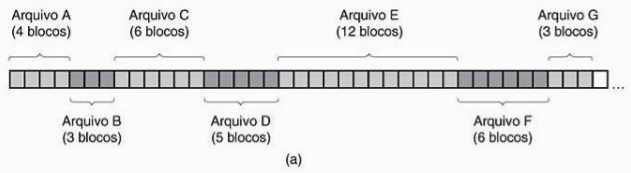
\includegraphics[width=.7\textwidth]{contiguous-alocation1}
    \caption{Arquivos alocados contiguamente}
  \end{subfigure}
  ~
  \begin{subfigure}{\textwidth}
    \centering
    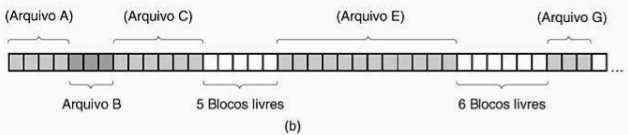
\includegraphics[width=.7\textwidth]{contiguous-alocation2}
    \caption{Disco fragmentado após exclusão dos arquivos $D$ e $F$}
  \end{subfigure}

  \caption{Esquema de alocação contígua no disco}
  \label{fig:contiguous-allocation}
\end{figure*}

\subsection{Lista Encadeada}
Aqui, os bloco continuam sendo mantidos como uma lista encadeada. Porém, na implementação, o ponteiro é colocado em uma tabela geral de blocos. Assim, cada bloco contém um ponteiro para um próximo bloco e o dado que ele carrega.

Esta técnica mitiga o problema da fragmentação, uma vez que arquivos não precisam ser guardados de forma sequencial. Porém, o acesso aleatório a dados é extremamente lento, uma vez que para ler um bloco qualquer, temos que ler todos os blocos que vem antes dele, dado que eles estão em uma lista encadeada.

\begin{figure}[h]
  \centering
  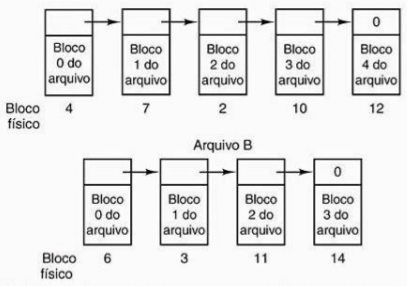
\includegraphics[width=.6\textwidth]{disk-file-list}
  \caption{Esquema de lista encadeada no disco}
  \label{fig:disk-file-list}
\end{figure}

\subsection{I-nodos}
Aqui, cada arquivo possui uma pequena tabela denominada de i-nodos, que contém os atributos e os endereços dos blocos físicos alocados ao arquivo. Os primeiros endereços de disco são armazenados no próprio i-nodo, que é transferido do disco para a memória no momento da abertura do arquivo.

Em arquivos maiores, o i-nodo contém o endereço de um bloco de disco denominado \textbf{bloco indireto simples}. Este bloco é uma tabela de endereços de blocos de disco, podendo haver indireção em segundo e terceiro níveis.

\section{Desempenho do Sistema de Arquivos}
Em geral, um acesso a disco é muito mais lento do que um acesso à memória principal. Uma maneira simples de aumentar a performance do sistema de arquivos é escrever e ler os dados da memória principal sempre que possível.

Para isso, necessitamos manter uma área de memória que armazenará temporariamente os blocos de disco mais utilizados. Como essa filosofia se assemelha à filosofia das \textit{caches} físicas, essa ára de memória chama-se \textbf{\textit{cache} de disco}, ou \textit{buffer cache}.

\begin{figure}[h]
  \centering
  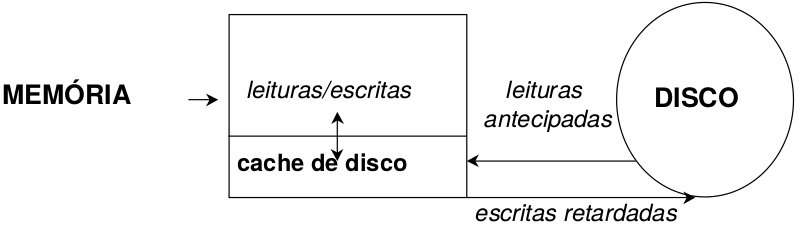
\includegraphics[width=.75\textwidth]{buffer-cache}
  \caption{Esquema geral de \textit{cache} de disco}
  \label{fig:buffer-cache}
\end{figure}

A gerência da \textit{cache} de disco necessita prever o que fazer quando a área reservada para a \textit{cache} estiver cheia. Da mesma maneira que um sistema paginado, devemos escolher um bloco para ser retirado da \textit{cache} de disco. Este problema, apesar de ser parecido com o da substituição de páginas, não deve ser resolvido da mesma maneira.

Além disso, A introdução da \textit{cache} de disco introduz um complicante na área de confiabilidade do sistema. Geralmente, uma operação de escrita em arquivo que retorna sucesso indica que o dado foi escrito no disco com sucesso. Em um sistema com \textit{cache} de disco, isso não é verdade, dado que este retorno simplesmente indica que o dado foi escrito na \textit{cache} de disco com sucesso. Logo, dados assumidos pelo usuário como escritos em disco podem ser perdidos após uma pane do sistema, por estarem em memória apenas.

Este problema se agrava quando os blocos alterados contém estruturas de controle do sistema de arquivos. Assim geralmente, os blocos são divididos em \textbf{blocos críticos} e \textbf{blocos de dados}. Os blocos críticos são sempre escritos na \textit{cache} de disco e no disco, gerando um \textit{bypass} da cache.

\begin{figure}[h]
  \centering
  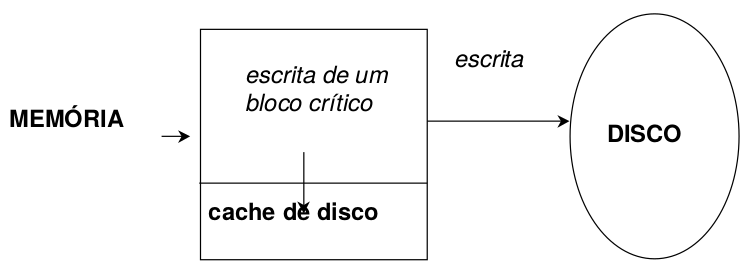
\includegraphics[width=0.75\textwidth]{buffer-cache-critic}
  \caption{\textit{Bypass} na escrita de blocos críticos}
  \label{fig:buffer-cache-critic}
\end{figure}
